\section{Block Coordinate Descent Algorithm} \label{ap:cgd}

We use a general purpose block coordinate descent algorithm (CGD)~\citep{tseng2009coordinate} to solve~\eqref{eq:estimator}. Following Tseng and Yun~\cite{tseng2009coordinate}, the complete CGD algorithm is given by Algorithm~\ref{alg:cgd}.

\begin{algorithm}[htbp]
	\caption{Coordinate Gradient Descent Algorithm to solve~\eqref{eq:estimator}} \label{alg:cgd}
\begin{algorithmic}[1]
\State	Set the iteration counter $k \leftarrow 0$ and choose initial values for the parameter vector $\bTheta^{(0)}$
\Repeat
\State Approximate the Hessian $\nabla^2 f(\bTheta^{(k)})$ by a symmetric matix $H^{(k)}$:
		\begin{equation}
			H^{(k)} = \diag \left[ \min \left\lbrace \max \left\lbrace \left[ \nabla^2 f(\bTheta^{(k)})\right] _{jj}, c_{min} \right\rbrace c_{max} \right\rbrace\right]_{j = 1, \ldots, p} \label{eq:Hk}
		\end{equation}
		\For{$ j =1, \ldots, p$}
\State	Solve the descent direction $d^{(k)} \coloneqq d_{H^{(k)}}(\Theta_{j}^{(k)})$ 
	\If{$\Theta_j^{(k)} \in \left\lbrace \beta_1, \ldots, \beta_p \right\rbrace$}
				\begin{equation}
					d_{H^{(k)}}(\Theta_{j}^{(k)}) \leftarrow \argmin_{d} \left\lbrace \nabla f(\Theta_{j}^{(k)}) d + \frac{1}{2} d^2 H^{(k)}_{j j} + \lambda P(\Theta_{j}^{(k)} + d) \right\rbrace \label{eq:descentdirection}
				\end{equation}
	\EndIf
%\If{$\Theta_j^{(k)} \in \left\lbrace \eta \right\rbrace$}
%	\begin{equation}
%					d_{H^{(k)}}(\Theta_{j}^{(k)}) \leftarrow - \nabla f(\Theta_{j}^{(k)}) / H_{jj}^{(k)}
%				\end{equation}
%\EndIf

\State Choose a stepsize
\begin{equation*}
	\alpha_j^{(k)} \leftarrow \tm{line search given by the Armijo rule}
\end{equation*}

\State Update
	\begin{equation*}
		\widehat{\Theta}_j^{(k+1)} \leftarrow \widehat{\Theta}_j^{(k)} + \alpha_j^{(k)}d^{(k)}
	\end{equation*}
\EndFor
\State Update
\begin{equation}
	\widehat\eta^{(k+1)} \leftarrow \argmin_{\eta}  \frac{1}{2} \sum_{i=1}^{N_T} \log(1 + \eta (\Lambda_i-1)) + \frac{1}{2{\sigma^2}^{\,(k)}} \sum_{i=1}^{N_T}\frac{\left(  \Ytilde_i - \sum_{j=0}^{p}\Xtilde_{ij+1}\beta_j^{(k+1)} \right) ^2}{1 + \eta (\Lambda_i-1)}
\end{equation}
\State Update
\begin{equation}
	%\widehat{\sigma^2}^{\,\,(k+1)} \leftarrow \frac{1}{N_T}\sum_{i=1}^{N_T}\frac{([ \bYtilde - \bXtilde \widehat{\bbeta}^{(k+1)}]_i )^2}{1 + \widehat{\eta}^{(k+1)} (\Lambda_i-1)}
	\widehat{\sigma^2}^{\,\,(k+1)} \gets \frac{1}{N_T}\sum_{i=1}^{N_T}\frac{\left(  \Ytilde_i - \sum_{j=0}^{p}\Xtilde_{ij+1}\beta_j^{(k+1)} \right) ^2}{1 + \eta^{(k+1)} (\Lambda_i-1)}
\end{equation}
\State $k \leftarrow k +1$
\State \Until{convergence criterion is satisfied}
\end{algorithmic}
\end{algorithm}

\begin{comment}
We note that conditional on $\widehat{\bbeta}$ and $\widehat{\eta}$, there exists an analytic solution for $\widehat{\sigma^2}$:
\begin{align}
	\frac{\partial}{\partial \sigma^2} f(\bTheta) &= \frac{N_T}{2\sigma^2}- \frac{1}{2\sigma^4} \sum_{i=1}^{N_T}\frac{([ \bYtilde - \bXtilde \bbeta]_i )^2}{1 + \eta (\Lambda_i-1)} = 0 \nonumber \\
	\widehat{\sigma^2} & = \frac{1}{N_T}\sum_{i=1}^{N_T}\frac{([ \bYtilde - \bXtilde \widehat{\bbeta}]_i )^2}{1 + \widehat{\eta} (\Lambda_i-1)} \label{eq:sigmahat}
\end{align}
\end{comment}

The Armijo rule is defined as follows~\citep{tseng2009coordinate}:
\begin{tcolorbox}
	Choose $\alpha_{init}^{(k)}>0$ and let $\alpha^{(k)}$ be the largest element of $\left\lbrace \alpha_{init}^k \delta^r \right\rbrace_{r = 0,1,2,\ldots} $ satisfying
	\begin{equation}
		Q_{\lambda}(\Theta_j^{(k)} + \alpha^{(k)} d^{(k)}) \leq Q_{\lambda} (\Theta_j^{(k)}) + \alpha^{(k)}\varrho \Delta^{(k)}
	\end{equation}
	where $0 < \delta <1$, $0 < \varrho <1$, $0 \leq \gamma < 1$ and
	\begin{equation}
		\Delta^{(k)} \coloneqq \nabla f(\Theta_j^{(k)})d^{(k)} + \gamma (d^{(k)})^2 H^{(k)}_{jj} + \lambda P(\Theta_j^{(k)} + d^{(k)}) - \lambda P(\Theta^{(k)})
	\end{equation}
\end{tcolorbox}
Common choices for the constants are $\delta=0.1$, $\varrho=0.001$, $\gamma = 0$, $\alpha_{init}^{(k)} = 1$ for all $k$~\citep{schelldorfer2011estimation}.

Below we detail the specifics of Algorithm~\ref{alg:cgd} for the $\ell_1$ penalty.

\subsection{$\ell_1$ penalty}\label{subsec:l1penalty}

The objective function is given by
\begin{equation}
	Q_{\lambda}(\bTheta) = f(\bTheta) + \lambda |\bbeta|
\end{equation}


\subsubsection{Descent Direction}
For simplicity, we remove the iteration counter $(k)$ from the derivation below.\\ For \mbox{$\Theta_j^{(k)} \in \left\lbrace \beta_1, \ldots, \beta_p \right\rbrace$}, let
\begin{equation}
	d_{H}(\Theta_{j}) = \argmin_{d} G(d)  \label{eq:argminGd}
\end{equation}
where
\[ G(d) =  \nabla f(\Theta_{j}) d + \frac{1}{2} d^2 H_{j j} + \lambda |\Theta_{j} + d| \]
Since $G(d)$ is not differentiable at $-\Theta_j$, we calculate the subdifferential $\partial G(d)$ and search for $d$ with $0 \in \partial G(d)$:
\begin{equation}
	\partial G(d) = \nabla f(\Theta_{j}) + d H_{j j} + \lambda u   \label{eq:subdiff}
\end{equation}
where
\begin{equation}
	u = \begin{cases}
		1 & \tm{if\quad}d > -\Theta_j \\
		-1 & \tm{if\quad} d < -\Theta_j\\
		[-1,1] & \tm{if\quad} d = \Theta_j
	\end{cases}
\end{equation}
We consider each of the three cases in~\eqref{eq:subdiff} below
\begin{enumerate}
	\item $d > -\Theta_j$
	\begin{align}
		\partial G(d) & = \nabla f(\Theta_{j}) + d H_{j j} + \lambda = 0 \nonumber \\
		d & = \frac{-(\nabla f(\Theta_{j}) + \lambda)}{H_{j j}}  \nonumber
	\end{align}
	Since $\lambda>0$ and $H_{jj}>0$, we have
	\begin{equation*}
		\frac{-(\nabla f(\Theta_{j}) - \lambda)}{H_{j j}} > \frac{-(\nabla f(\Theta_{j}) + \lambda)}{H_{j j}} = d \overset{\tm{def}}{>} -\Theta_j
	\end{equation*}
	The solution can be written compactly as
	\begin{equation*}
		d = \tm{mid}\left\lbrace \frac{-(\nabla f(\Theta_{j}) - \lambda)}{H_{j j}}, -\Theta_j ,\frac{-(\nabla f(\Theta_{j}) + \lambda)}{H_{j j}} \right\rbrace
	\end{equation*}
	where $\tm{mid}\left\lbrace a,b,c \right\rbrace$ denotes the median (mid-point) of $a,b,c$~\citep{tseng2009coordinate}.
	\item $d < -\Theta_j$
	\begin{align}
		\partial G(d) & = \nabla f(\Theta_{j}) + d H_{j j} - \lambda = 0 \nonumber \\
		d & = \frac{-(\nabla f(\Theta_{j}) - \lambda)}{H_{j j}}  \nonumber
	\end{align}
	Since $\lambda>0$ and $H_{jj}>0$, we have
	\begin{equation*}
		\frac{-(\nabla f(\Theta_{j}) + \lambda)}{H_{j j}} < \frac{-(\nabla f(\Theta_{j}) - \lambda)}{H_{j j}} = d \overset{\tm{def}}{<} -\Theta_j
	\end{equation*}
	Again, the solution can be written compactly as
	\begin{equation*}
		d = \tm{mid}\left\lbrace \frac{-(\nabla f(\Theta_{j}) - \lambda)}{H_{j j}}, -\Theta_j ,\frac{-(\nabla f(\Theta_{j}) + \lambda)}{H_{j j}} \right\rbrace
	\end{equation*}
	
	\item $d_j = -\Theta_j$\\
	There exists $u \in [-1,1]$ such that
	\begin{align*}
		\partial G(d) & = \nabla f(\Theta_{j}) + d H_{j j} + \lambda u = 0 \nonumber \\
		d & = \frac{-(\nabla f(\Theta_{j}) + \lambda u)}{H_{j j}}  \nonumber
	\end{align*}
	For $-1 \leq u \leq 1$, $\lambda>0$ and $H_{jj}>0$ we have
	\begin{equation*}
		\frac{-(\nabla f(\Theta_{j}) + \lambda)}{H_{j j}} \leq  d \overset{\tm{def}}{=} -\Theta_j \leq \frac{-(\nabla f(\Theta_{j}) - \lambda)}{H_{j j}}
	\end{equation*}
	The solution can again be written compactly as
	\begin{equation*}
		d = \tm{mid}\left\lbrace \frac{-(\nabla f(\Theta_{j}) - \lambda)}{H_{j j}}, -\Theta_j ,\frac{-(\nabla f(\Theta_{j}) + \lambda)}{H_{j j}} \right\rbrace
	\end{equation*}
	
\end{enumerate}
We see all three cases lead to the same solution for~\eqref{eq:argminGd}. Therefore the descent direction for $\Theta_j^{(k)} \in \left\lbrace \beta_1, \ldots, \beta_p \right\rbrace$ for the $\ell_1$ penalty is given by
\begin{equation}
	d = \tm{mid}\left\lbrace \frac{-(\nabla f(\beta_{j}) - \lambda)}{H_{j j}}, -\beta_j ,\frac{-(\nabla f(\beta_{j}) + \lambda)}{H_{j j}} \right\rbrace  \label{eq:d}
\end{equation}

\subsubsection{Solution for the $\beta$ parameter} \label{ap:beta}
If the Hessian $\nabla^2f(\bTheta^{(k)}) >0$ then $H^{(k)}$ defined in~\eqref{eq:Hk} is equal to $\nabla^2f(\bTheta^{(k)})$. Using $\alpha_{init} = 1$, the largest element of $\left\lbrace \alpha_{init}^{(k)} \delta^r \right\rbrace_{r = 0, 1, 2, \ldots}$ satisfying the Armijo Rule inequality is reached for $\alpha^{(k)} = \alpha_{init}^{(k)}\delta^0 = 1$. The Armijo rule update for the $\bbeta$ parameter is then given by
\begin{equation}
	\beta_j^{(k+1)} \leftarrow \beta_j^{(k)} + d^{(k)}, \qquad j=1, \ldots, p \label{eq:betaupdate}
\end{equation}
Substituting the descent direction given by~\eqref{eq:d} into~\eqref{eq:betaupdate} we get
\begin{equation}
	\beta_j^{(k+1)} = \tm{mid}\left\lbrace \beta_j^{(k)}+ \frac{-(\nabla f(\beta_j^{(k)}) - \lambda)}{H_{j j}}, 0,\beta_j^{(k)}+ \frac{-(\nabla f(\beta_j^{(k)}) + \lambda)}{H_{j j}}  \right\rbrace \label{eq:betaMidpoint}
\end{equation}
We can further simplify this expression. Let %Let $\bXtilde_{-j}$ and $\bbeta^{(k)}_{-j}$ correspond to $\bXtilde$ and $\bbeta^{(k)}$ without the $j^{\tm{th}}$ variable, respectively. Furthermore, let

\begin{equation}
	w_i \coloneqq \frac{1}{\sigma^2\left(1+\eta(\Lambda_i-1)\right)}
\end{equation}.


Re-write the part depending on $\bbeta$ of the negative log-likelihood in~\eqref{eq:LikeFinal} as
\begin{align}
	%\frac{1}{2\sigma^2} \sum_{i=1}^{N_T}\frac{\left(  \Ytilde_i - \sum_{j=1}^{p}\Xtilde_{ij}\beta_j^{(k)} \right) ^2}{1 + \eta (\Lambda_i-1)}
	g(\bbeta^{(k)}) & = \frac{1}{2} \sum_{i=1}^{N_T} w_i\left(  \Ytilde_i - \sum_{\ell \neq j}\Xtilde_{i\ell} \beta_\ell^{(k)} - \Xtilde_{ij}\beta_j^{(k)} \right) ^2
\end{align}
The gradient and Hessian are given by
\begin{align}
	\nabla f(\beta_j^{(k)}) \coloneqq \frac{\partial}{\partial \beta_j^{(k)}}g(\bbeta^{(k)}) & = - \sum_{i=1}^{N_T} w_i \Xtilde_{ij}\left(  \Ytilde_i - \sum_{\ell \neq j}\Xtilde_{i\ell} \beta_\ell^{(k)} - \Xtilde_{ij}\beta_j^{(k)} \right)  \label{eq:grad}\\
	H_{jj} \coloneqq \frac{\partial^2}{\partial {\beta_j^{(k)}}^2}g(\bbeta^{(k)}) & = \sum_{i=1}^{N_T} w_i \Xtilde_{ij}^2  \label{eq:hessian}
\end{align}
Substituting~\eqref{eq:grad} and~\eqref{eq:hessian} into $\beta_j^{(k)}+ \frac{-(\nabla f(\beta_j^{(k)}) - \lambda)}{H_{jj}}$ %~\eqref{eq:betaMidpoint} we get
\begin{align}
	& \beta_j^{(k)}+ \frac{  \sum_{i=1}^{N_T} w_i \Xtilde_{ij}\left(  \Ytilde_i - \sum_{\ell \neq j}\Xtilde_{i\ell} \beta_\ell^{(k)} - \Xtilde_{ij}\beta_j^{(k)} \right)  + \lambda }{\sum_{i=1}^{N_T} w_i \Xtilde_{ij}^2} \nonumber \\
	& = \beta_j^{(k)}+ \frac{ \sum_{i=1}^{N_T} w_i \Xtilde_{ij}\left(  \Ytilde_i - \sum_{\ell \neq j}\Xtilde_{i\ell} \beta_\ell^{(k)} \right) + \lambda}{\sum_{i=1}^{N_T} w_i \Xtilde_{ij}^2} - \frac{\sum_{i=1}^{N_T} w_i \Xtilde_{ij}^2\beta_j^{(k)}  }{\sum_{i=1}^{N_T} w_i \Xtilde_{ij}^2} \nonumber \\
	& =  \frac{  \sum_{i=1}^{N_T} w_i \Xtilde_{ij}\left(  \Ytilde_i - \sum_{\ell \neq j}\Xtilde_{i\ell} \beta_\ell^{(k)} \right) + \lambda}{\sum_{i=1}^{N_T} w_i \Xtilde_{ij}^2} \label{eq:midleft}
\end{align}
Similarly, substituting~\eqref{eq:grad} and~\eqref{eq:hessian} in $\beta_j^{(k)}+ \frac{-(\nabla f(\beta_j^{(k)}) + \lambda)}{H_{jj}}$ we get
\begin{align}
	\frac{  \sum_{i=1}^{N_T} w_i \Xtilde_{ij}\left(  \Ytilde_i - \sum_{\ell \neq j}\Xtilde_{i\ell} \beta_\ell^{(k)} \right) - \lambda}{\sum_{i=1}^{N_T} w_i \Xtilde_{ij}^2} \label{eq:midright}
\end{align}
Finally, substituting~\eqref{eq:midleft} and~\eqref{eq:midright} into~\eqref{eq:betaMidpoint} we get
\begin{align}
	\beta_j^{(k+1)} & = \tm{mid}\left\lbrace \frac{  \sum_{i=1}^{N_T} w_i \Xtilde_{ij}\left(  \Ytilde_i - \sum_{\ell \neq j}\Xtilde_{i\ell} \beta_\ell^{(k)} \right) - \lambda}{\sum_{i=1}^{N_T} w_i \Xtilde_{ij}^2}, 0,\frac{  \sum_{i=1}^{N_T} w_i \Xtilde_{ij}\left(  \Ytilde_i - \sum_{\ell \neq j}\Xtilde_{i\ell} \beta_\ell^{(k)} \right) + \lambda}{\sum_{i=1}^{N_T} w_i \Xtilde_{ij}^2} \right\rbrace \nonumber \\
	& = \frac{\mathcal{S}_{\lambda}\left( \sum_{i=1}^{N_T} w_i \Xtilde_{ij}\left(  \Ytilde_i - \sum_{\ell \neq j}\Xtilde_{i\ell} \beta_\ell^{(k)} \right)\right) }{\sum_{i=1}^{N_T} w_i \Xtilde_{ij}^2} \label{eq:betaUpdateSoft}
\end{align}

Where $\mathcal{S}_{\lambda}(x)$ is the soft-thresholding operator
\begin{equation*}
	\mathcal{S}_{\lambda}(x) = \tm{sign}(x)(|x| - \lambda)_+
\end{equation*}
$\textrm{sign}(x)$ is the signum function
\begin{equation*}
	\textrm{sign}(x) = \begin{cases}
		-1 & x<0\\
		0 & x= 0\\
		1 & x>0
	\end{cases}
\end{equation*}
and $(x)_+ = \max(x, 0)$.

%We note that the parameter update for $\beta_j$ given by~\eqref{eq:betaUpdateSoft} takes the same form as the weighted updates of the \texttt{glmnet} algorithm~\citep{friedman2010regularization} (Section 2.4, equation (10)) with $\alpha=1$.


\FloatBarrier 

\newpage

\section{Additional Simulation Results} \label{ap:ggmix_sim_results}

\begin{knitrout}\scriptsize
\definecolor{shadecolor}{rgb}{0.969, 0.969, 0.969}\color{fgcolor}\begin{figure}[H]

{\centering 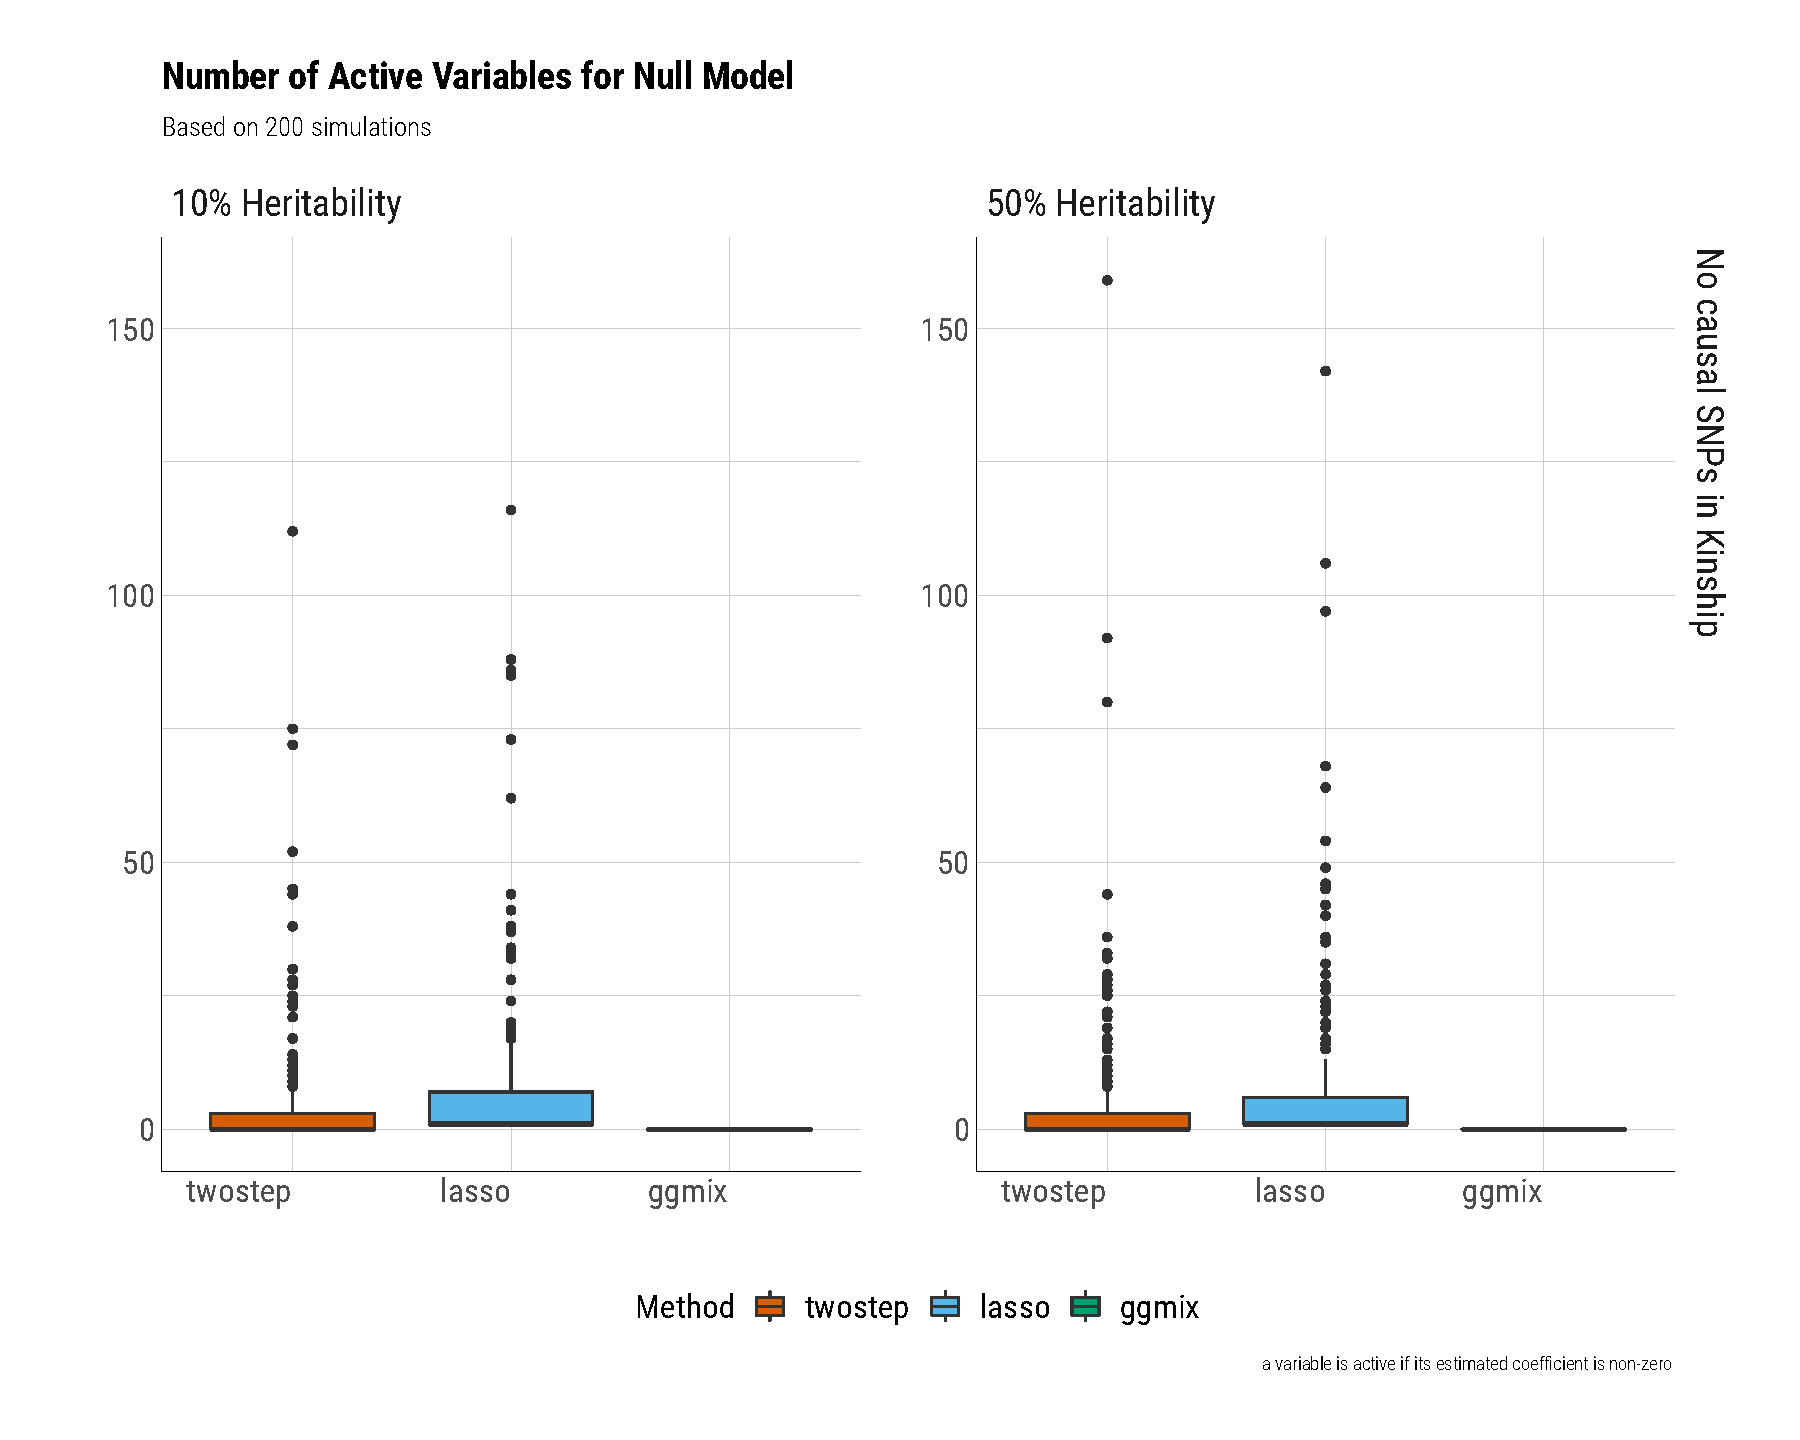
\includegraphics[width=1\linewidth]{figs/plot-nactive-sim-null-model-1} 

}

\caption[Boxplots of the number of active variables from 200 simulations by the true heritability $\eta = \lbrace 10\%, 50\% \rbrace$ for the null model ($c=0$)]{Boxplots of the number of active variables from 200 simulations by the true heritability $\eta = \lbrace 10\%, 50\% \rbrace$ for the null model ($c=0$).}\label{fig:plot-nactive-sim-null-model}
\end{figure}


\end{knitrout}


\begin{knitrout}\scriptsize
\definecolor{shadecolor}{rgb}{0.969, 0.969, 0.969}\color{fgcolor}\begin{figure}[H]

{\centering 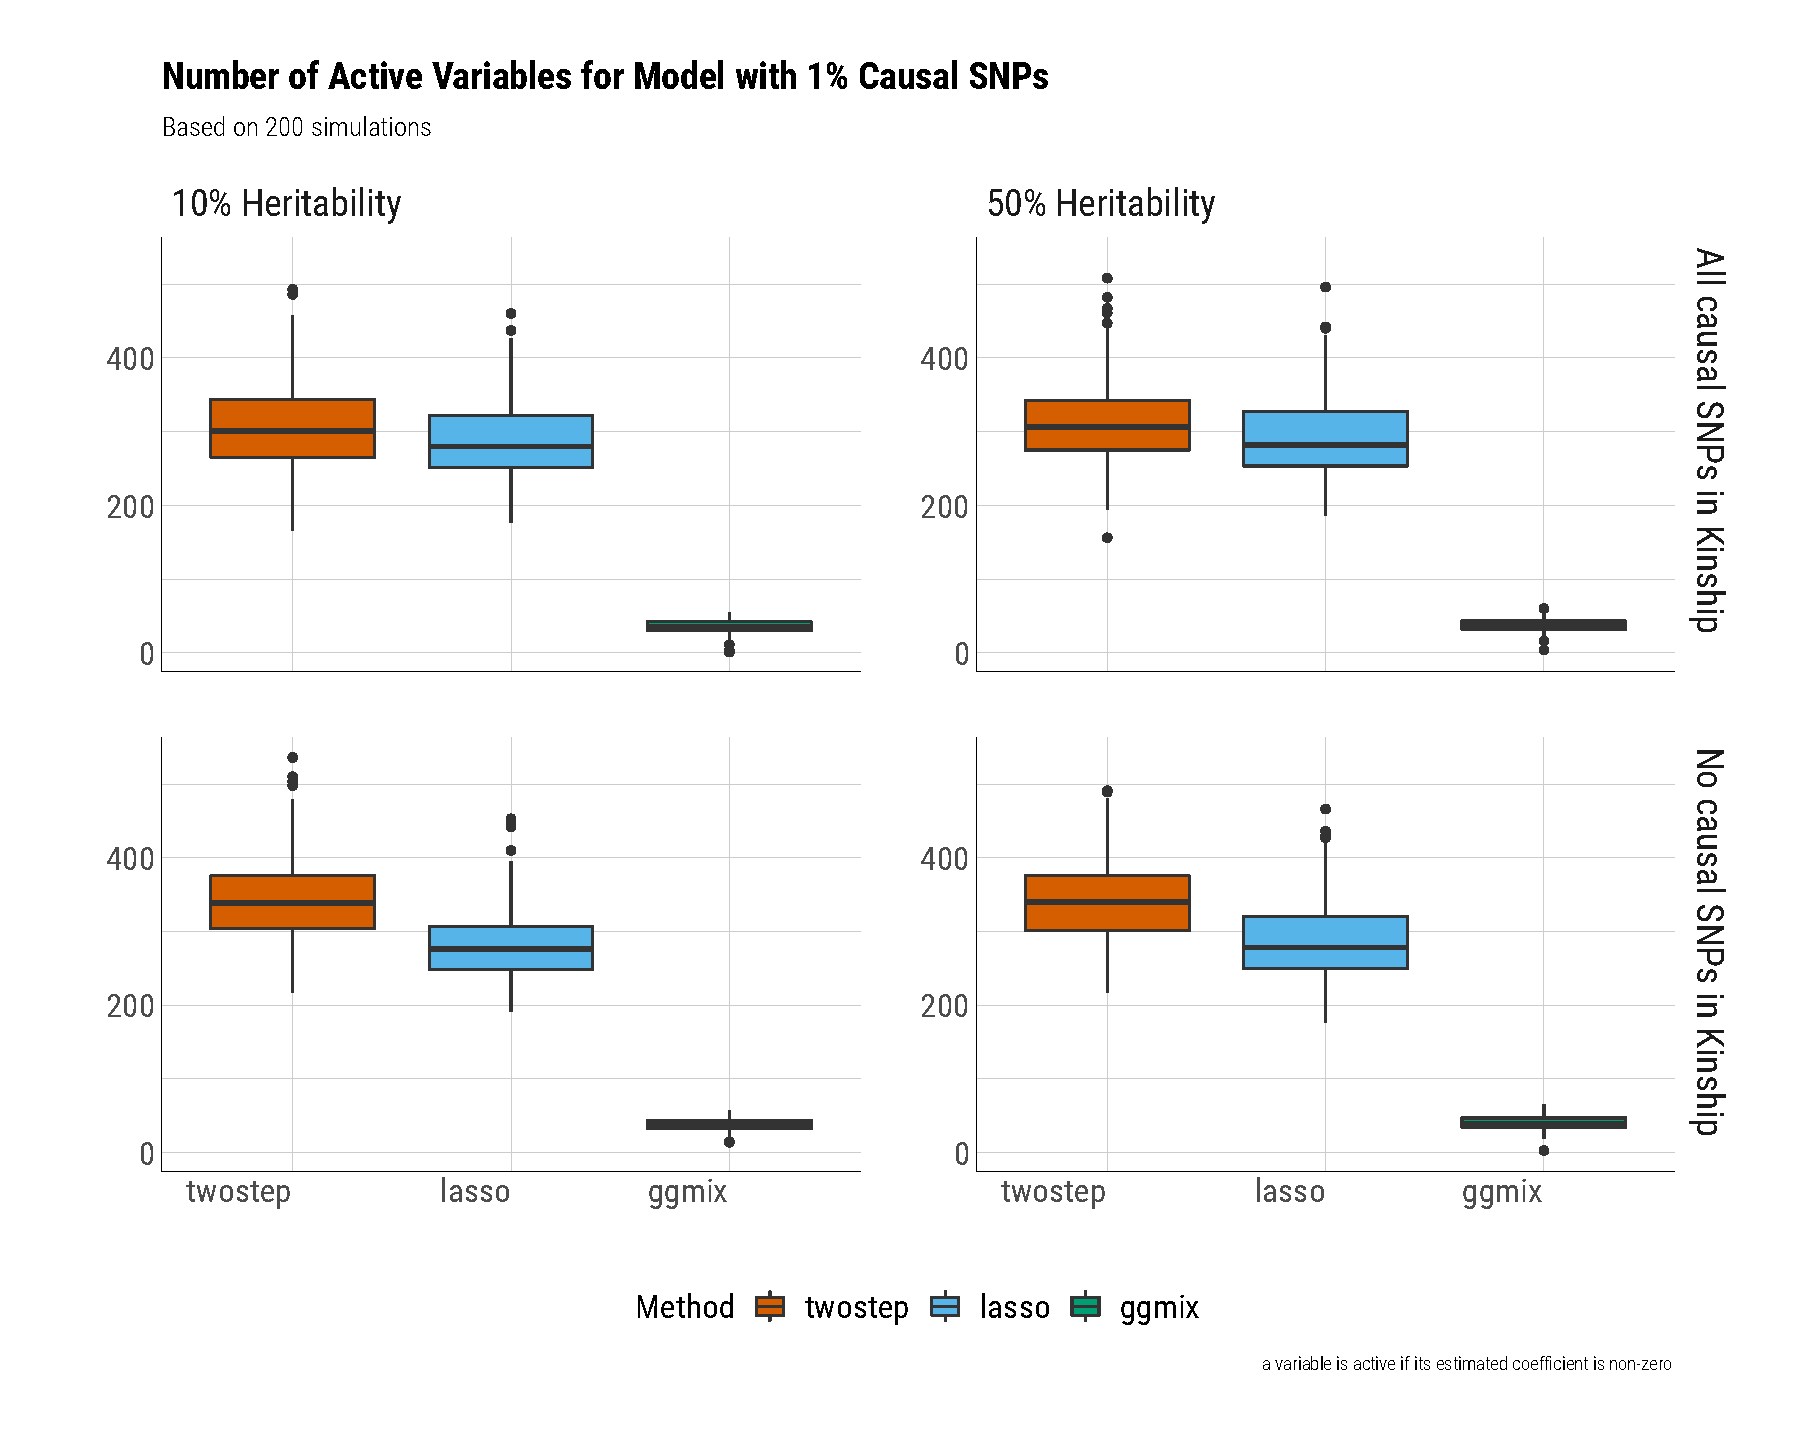
\includegraphics[width=1\linewidth]{figs/plot-nactive-sim-1p-causal-1} 

}

\caption[Boxplots of the number of active variables from 200 simulations by the true heritability $\eta = \lbrace 10\%, 50\% \rbrace$ and number of causal SNPs that were included in the calculation of the kinship matrix for the model with 1\% causal SNPs ($c=0.01$)]{Boxplots of the number of active variables from 200 simulations by the true heritability $\eta = \lbrace 10\%, 50\% \rbrace$ and number of causal SNPs that were included in the calculation of the kinship matrix for the model with 1\% causal SNPs ($c=0.01$).}\label{fig:plot-nactive-sim-1p-causal}
\end{figure}


\end{knitrout}

\begin{knitrout}\scriptsize
\definecolor{shadecolor}{rgb}{0.969, 0.969, 0.969}\color{fgcolor}\begin{figure}[H]

{\centering 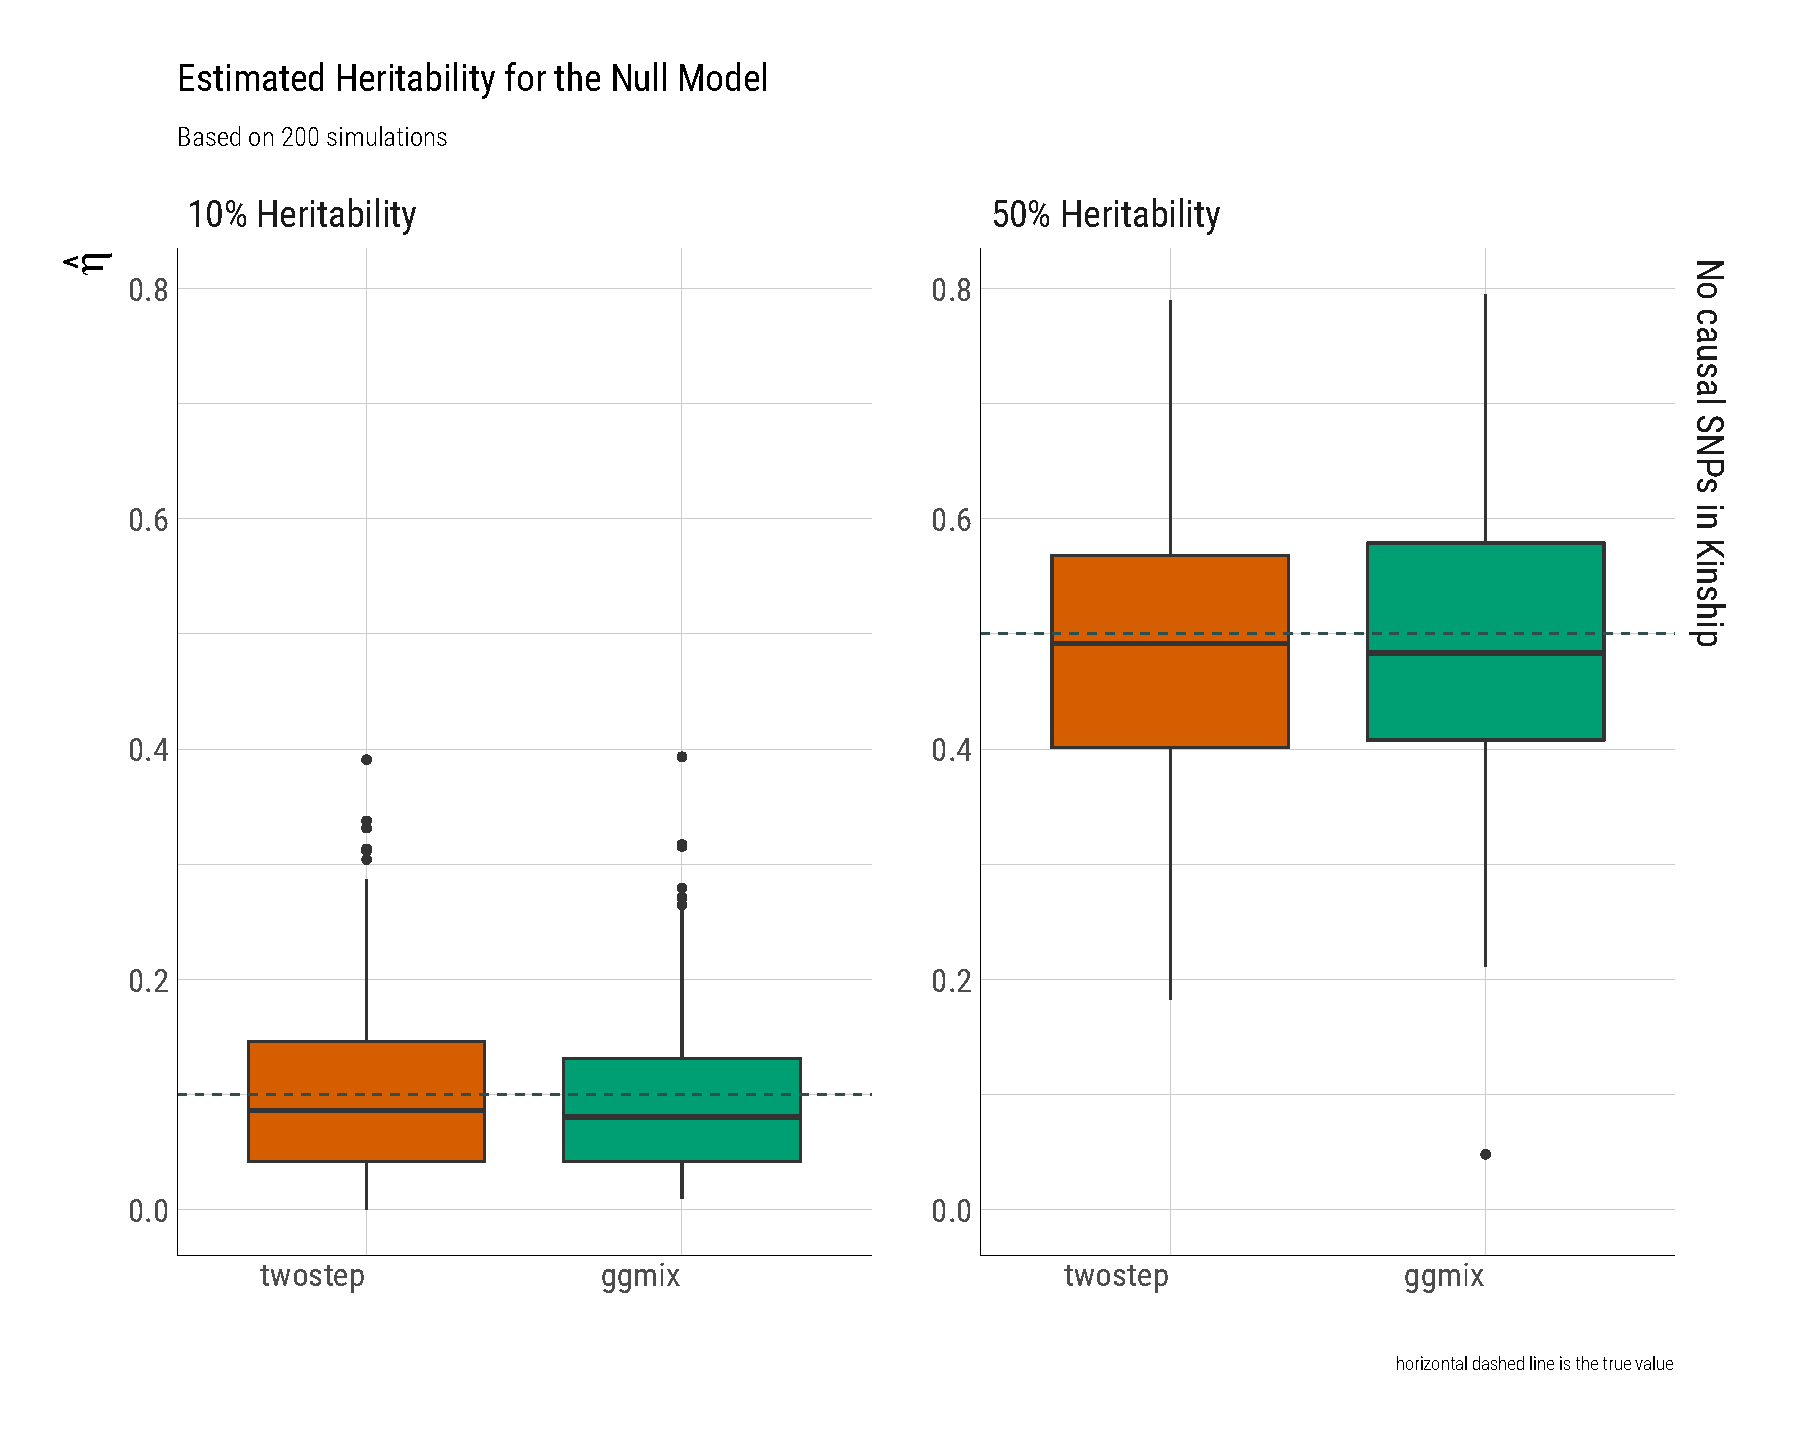
\includegraphics[width=1\linewidth]{figs/plot-eta-sim-null-model-1} 

}

\caption[Boxplots of the heritability estimate $\hat{\eta}$ from 200 simulations by the true heritability $\eta = \lbrace 10\%, 50\% \rbrace$ for the null model ($c=0$)]{Boxplots of the heritability estimate $\hat{\eta}$ from 200 simulations by the true heritability $\eta = \lbrace 10\%, 50\% \rbrace$ for the null model ($c=0$).}\label{fig:plot-eta-sim-null-model}
\end{figure}


\end{knitrout}

\begin{knitrout}\scriptsize
\definecolor{shadecolor}{rgb}{0.969, 0.969, 0.969}\color{fgcolor}\begin{figure}[H]

{\centering 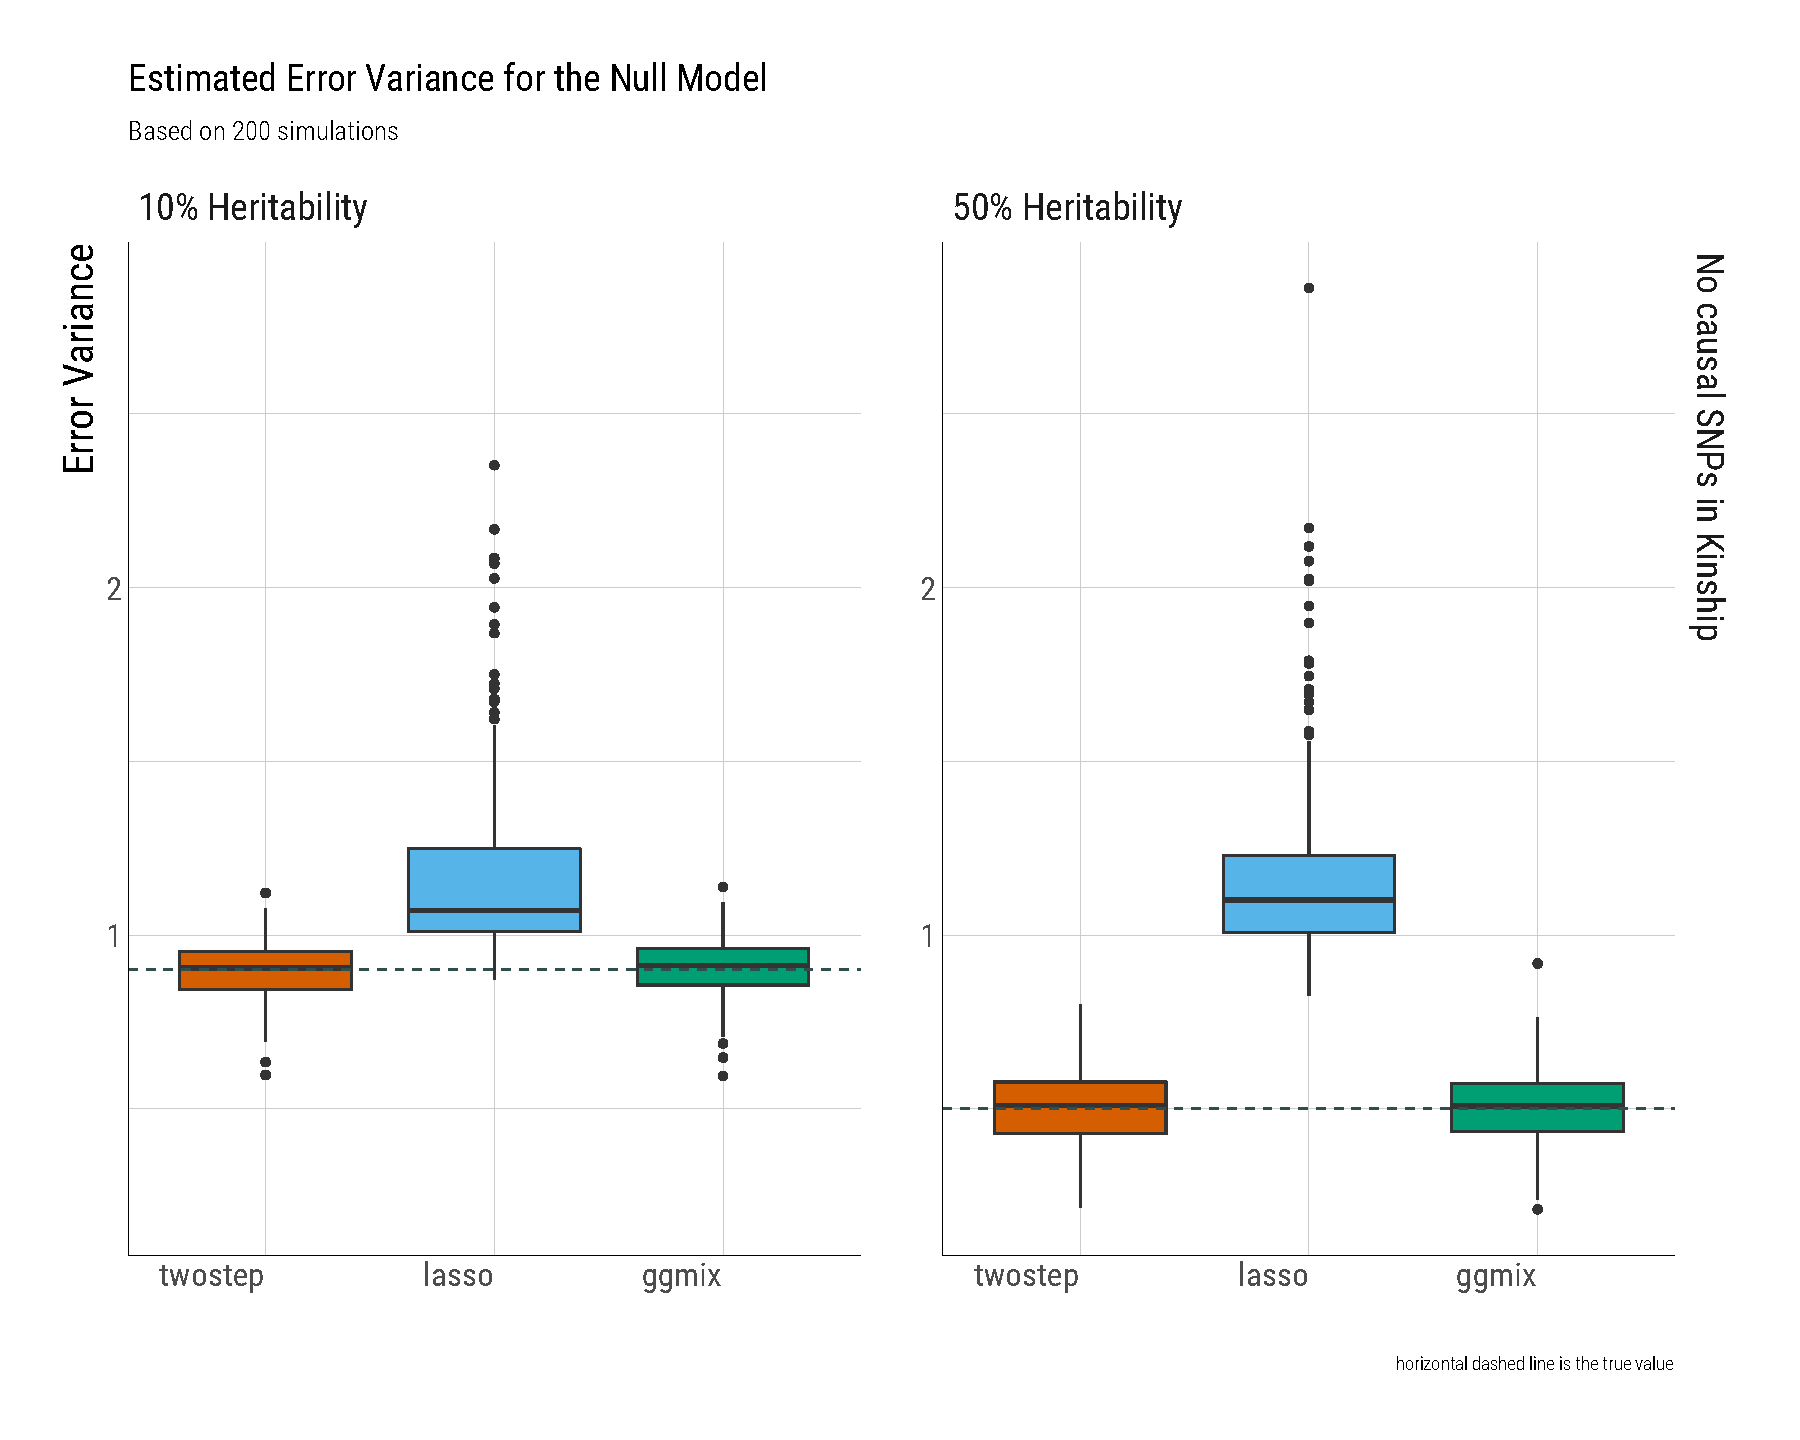
\includegraphics[width=1\linewidth]{figs/plot-errorvar-sim-null-model-1} 

}

\caption[Boxplots of the estimated error variance from 200 simulations by the true heritability $\eta = \lbrace 10\%, 50\% \rbrace$ for the null model ($c=0$)]{Boxplots of the estimated error variance from 200 simulations by the true heritability $\eta = \lbrace 10\%, 50\% \rbrace$ for the null model ($c=0$).}\label{fig:plot-errorvar-sim-null-model}
\end{figure}


\end{knitrout}

\begin{knitrout}\scriptsize
\definecolor{shadecolor}{rgb}{0.969, 0.969, 0.969}\color{fgcolor}\begin{figure}[H]

{\centering 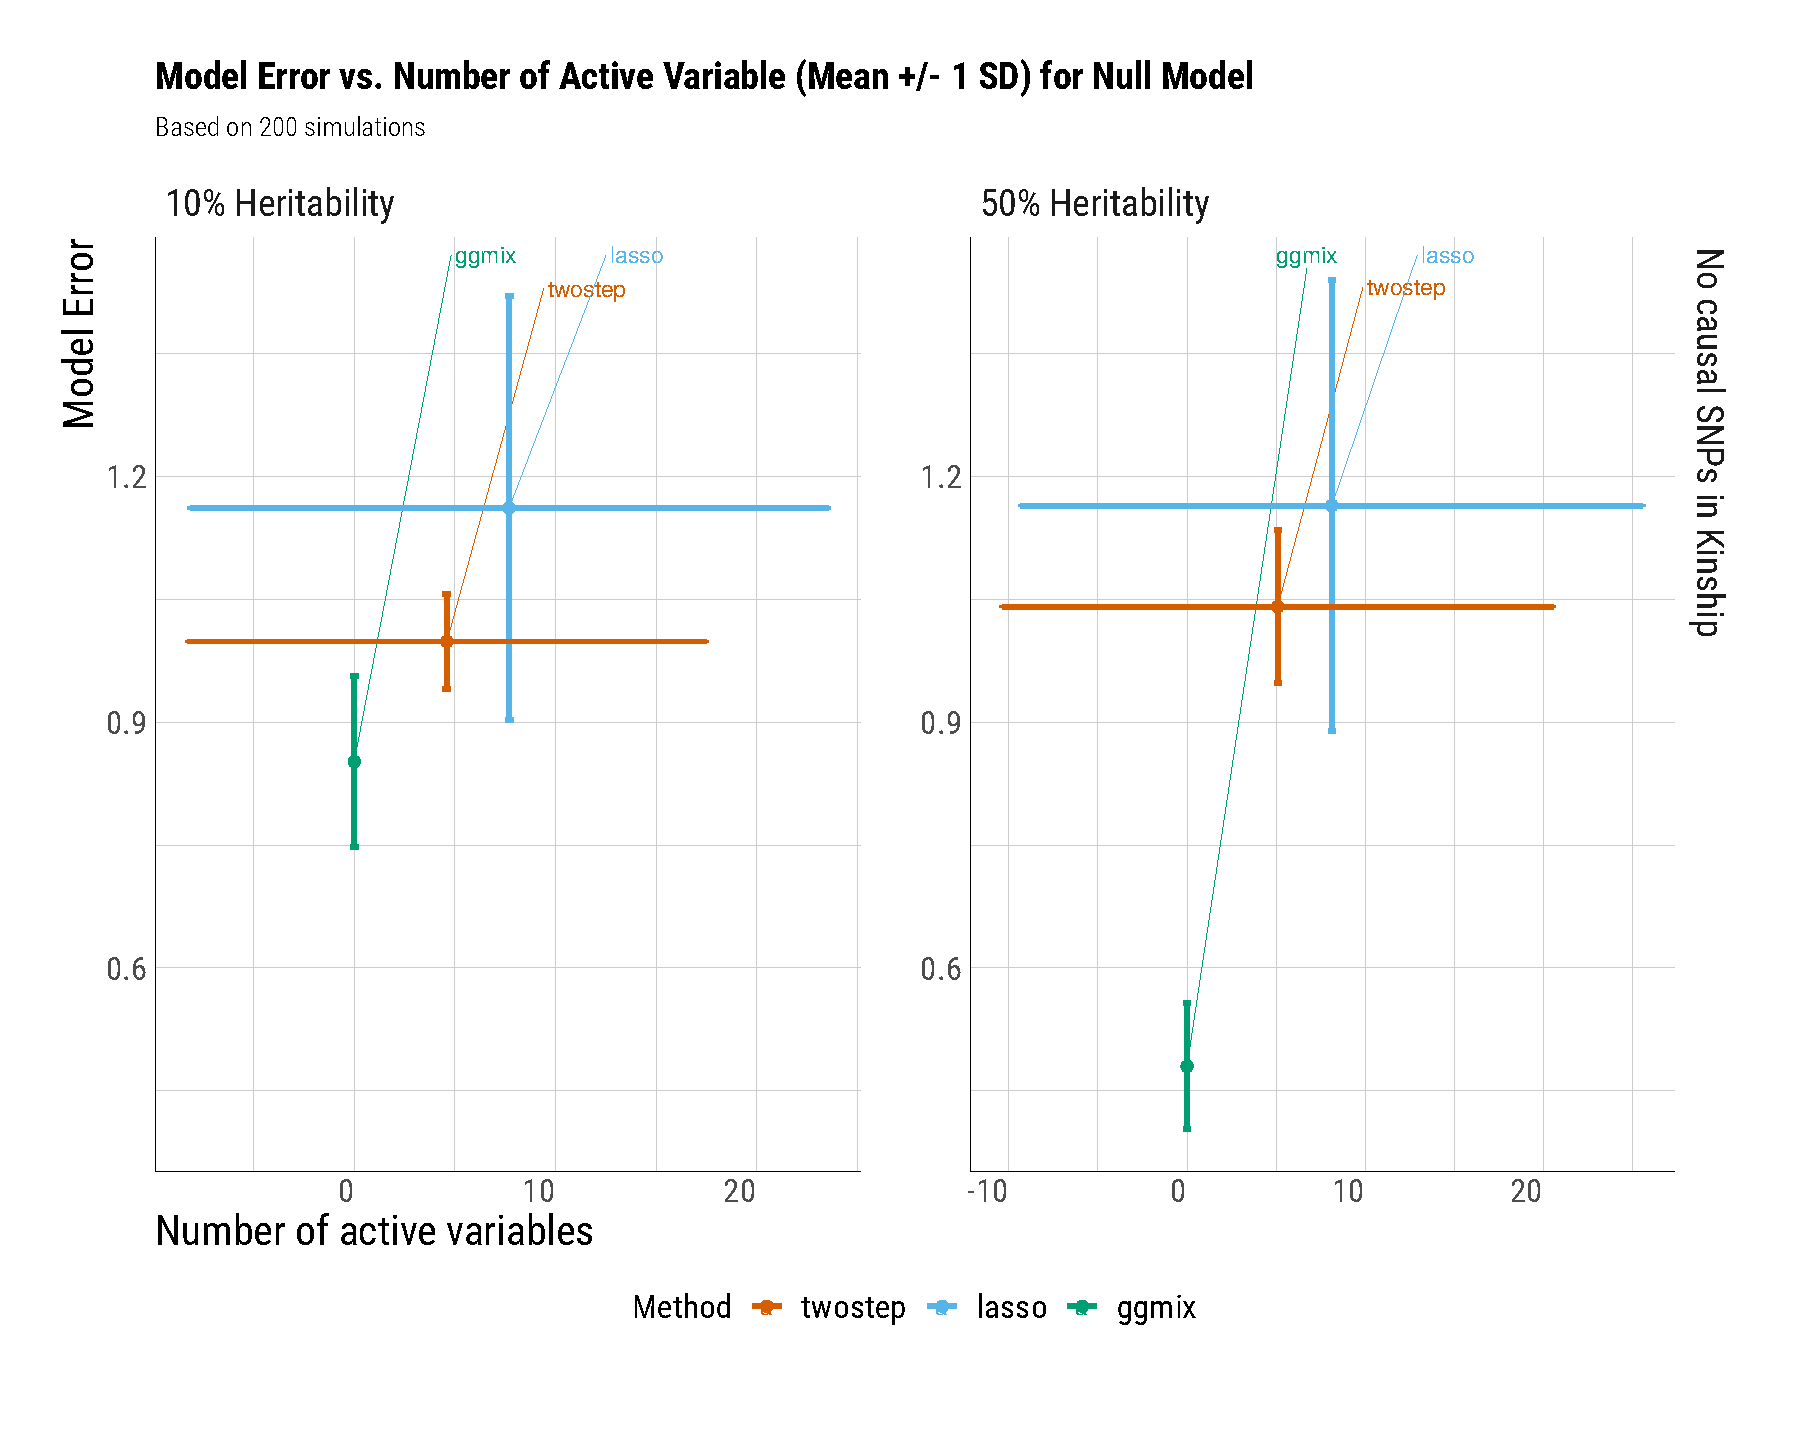
\includegraphics[width=1\linewidth]{figs/plot-me-nactive-sim-null-1} 

}

\caption[Means $\pm 1$ standard deviation of the model error vs]{Means $\pm 1$ standard deviation of the model error vs. the number of active variables by the true heritability $\eta = \lbrace 10\%, 50\% \rbrace$ for the null model ($c=0$).}\label{fig:plot-me-nactive-sim-null}
\end{figure}


\end{knitrout}

\FloatBarrier 

\newpage


\section{\ggmix ~Package Showcase} \label{ap:showcase}

In this section we briefly introduce the freely available and open source \ggmix ~package in \texttt{R}. More comprehensive documentation is available at \url{https://sahirbhatnagar.com/ggmix}. Note that this entire section is reproducible; the code and text are combined in an \texttt{.Rnw}\footnote[1]{scripts available at \url{https://github.com/sahirbhatnagar/ggmix/tree/master/manuscript}} file and compiled using \texttt{knitr}~\citep{xie2015dynamic}. 

\subsection{Installation}

The package can be installed from \href{https://github.com/sahirbhatnagar/ggmix}{GitHub} via


\begin{knitrout}\scriptsize
\definecolor{shadecolor}{rgb}{0.969, 0.969, 0.969}\color{fgcolor}\begin{kframe}
\begin{alltt}
\hlkwd{install.packages}\hlstd{(}\hlstr{"pacman"}\hlstd{)}
\hlstd{pacman}\hlopt{::}\hlkwd{p_load_gh}\hlstd{(}\hlstr{'sahirbhatnagar/ggmix'}\hlstd{)}
\end{alltt}
\end{kframe}
\end{knitrout}

To showcase the main functions in \ggmix, ~we will use the simulated data which ships with the package and can be loaded via:

\begin{knitrout}\scriptsize
\definecolor{shadecolor}{rgb}{0.969, 0.969, 0.969}\color{fgcolor}\begin{kframe}
\begin{alltt}
\hlkwd{library}\hlstd{(ggmix)}
\hlkwd{data}\hlstd{(}\hlstr{"admixed"}\hlstd{)}
\hlkwd{names}\hlstd{(admixed)}
\end{alltt}
\begin{verbatim}
##  [1] "y"               "x"               "causal"         
##  [4] "beta"            "kin"             "Xkinship"       
##  [7] "not_causal"      "causal_positive" "causal_negative"
## [10] "x_lasso"
\end{verbatim}
\end{kframe}
\end{knitrout}

For details on how this data was simulated, see \texttt{help(admixed)}.  

There are three basic inputs that \ggmix ~needs:  
\begin{enumerate}
	\item $Y$: a continuous response variable  
\item $X$: a matrix of covariates of dimension $N \times p$ where $N$ is the sample size and $p$ is the number of covariates  
\item $\boldsymbol{\Phi}$: a kinship matrix  
\end{enumerate}

We can visualize the kinship matrix in the \texttt{admixed} data using the \texttt{popkin} package:  

\begin{knitrout}\scriptsize
\definecolor{shadecolor}{rgb}{0.969, 0.969, 0.969}\color{fgcolor}\begin{kframe}
\begin{alltt}
\hlcom{# need to install the package if you don't have it}
\hlcom{# pacman::p_load_gh('StoreyLab/popkin')}
\hlstd{popkin}\hlopt{::}\hlkwd{plotPopkin}\hlstd{(admixed}\hlopt{$}\hlstd{kin)}
\end{alltt}
\end{kframe}

{\centering 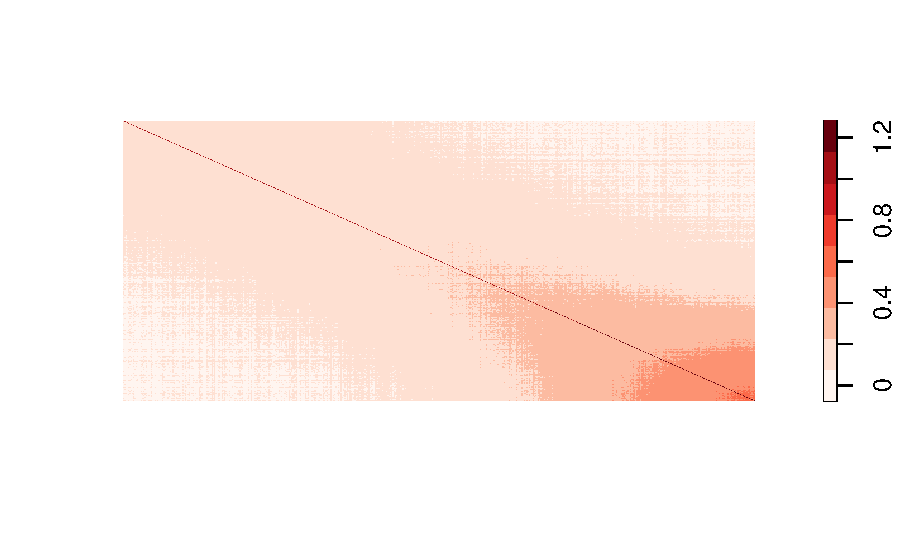
\includegraphics[width=1\linewidth]{figs/ggmix-popkin-1} 

}



\end{knitrout}

\subsection{Fit the linear mixed model with Lasso Penalty}

We will use the most basic call to the main function of this package, which is called \texttt{ggmix}. This function will by default fit a $L_1$ penalized linear mixed model (LMM) for 100 distinct values of the tuning parameter $\lambda$. It will choose its own sequence:  

\begin{knitrout}\scriptsize
\definecolor{shadecolor}{rgb}{0.969, 0.969, 0.969}\color{fgcolor}\begin{kframe}
\begin{alltt}
\hlstd{fit} \hlkwb{<-} \hlkwd{ggmix}\hlstd{(}\hlkwc{x} \hlstd{= admixed}\hlopt{$}\hlstd{x,} \hlkwc{y} \hlstd{= admixed}\hlopt{$}\hlstd{y,} \hlkwc{kinship} \hlstd{= admixed}\hlopt{$}\hlstd{kin)}
\hlkwd{names}\hlstd{(fit)}
\end{alltt}
\begin{verbatim}
##  [1] "result"       "ggmix_object" "n_design"     "p_design"    
##  [5] "lambda"       "coef"         "b0"           "beta"        
##  [9] "df"           "eta"          "sigma2"       "nlambda"     
## [13] "cov_names"    "call"
\end{verbatim}
\begin{alltt}
\hlkwd{class}\hlstd{(fit)}
\end{alltt}
\begin{verbatim}
## [1] "lassofullrank" "ggmix_fit"
\end{verbatim}
\end{kframe}
\end{knitrout}

We can see the solution path for each variable by calling the \texttt{plot} method for objects of class \texttt{ggmix\_fit}:  

\begin{knitrout}\scriptsize
\definecolor{shadecolor}{rgb}{0.969, 0.969, 0.969}\color{fgcolor}\begin{kframe}
\begin{alltt}
\hlkwd{plot}\hlstd{(fit)}
\end{alltt}
\end{kframe}

{\centering 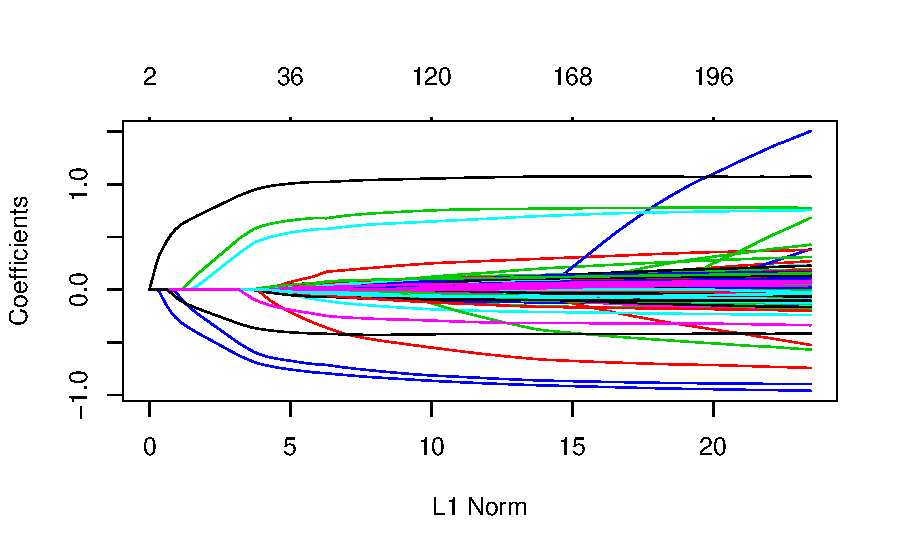
\includegraphics[width=1\linewidth]{figs/ggmix-solution-path-1} 

}



\end{knitrout}

We can also get the coefficients for given value(s) of lambda using the \texttt{coef} method for objects of class \texttt{ggmix\_fit}:  

\begin{knitrout}\scriptsize
\definecolor{shadecolor}{rgb}{0.969, 0.969, 0.969}\color{fgcolor}\begin{kframe}
\begin{alltt}
\hlcom{# only the first 5 coefficients printed here for brevity}
\hlkwd{coef}\hlstd{(fit,} \hlkwc{s} \hlstd{=} \hlkwd{c}\hlstd{(}\hlnum{0.1}\hlstd{,}\hlnum{0.02}\hlstd{))[}\hlnum{1}\hlopt{:}\hlnum{5}\hlstd{, ]}
\end{alltt}
\begin{verbatim}
## 5 x 2 Matrix of class "dgeMatrix"
##                      1            2
## (Intercept) -0.3824525 -0.030227753
## X62          0.0000000  0.000000000
## X185         0.0000000  0.001444670
## X371         0.0000000  0.009513604
## X420         0.0000000  0.000000000
\end{verbatim}
\end{kframe}
\end{knitrout}
Here, \texttt{s} specifies the value(s) of $\lambda$ at which the extraction is made. The function uses linear interpolation to make predictions for values of \texttt{s} that do not coincide with the lambda sequence used in the fitting algorithm.  

We can also get predictions ($X\widehat{\boldsymbol{\beta}}$) using the \texttt{predict} method for objects of class \texttt{ggmix\_fit}:  

\begin{knitrout}\scriptsize
\definecolor{shadecolor}{rgb}{0.969, 0.969, 0.969}\color{fgcolor}\begin{kframe}
\begin{alltt}
\hlcom{# need to provide x to the predict function}
\hlcom{# predict for the first 5 subjects }
\hlkwd{predict}\hlstd{(fit,} \hlkwc{s} \hlstd{=} \hlkwd{c}\hlstd{(}\hlnum{0.1}\hlstd{,}\hlnum{0.02}\hlstd{),} \hlkwc{newx} \hlstd{= admixed}\hlopt{$}\hlstd{x[}\hlnum{1}\hlopt{:}\hlnum{5}\hlstd{,])}
\end{alltt}
\begin{verbatim}
##               1          2
## id1 -1.19165061 -1.3123396
## id2 -0.02913052  0.3885921
## id3 -2.00084875 -2.6460045
## id4 -0.37255277 -0.9542455
## id5 -1.03967831 -2.1377274
\end{verbatim}
\end{kframe}
\end{knitrout}


\subsection{Find the Optimal Value of the Tuning Parameter}

We use the Generalized Information Criterion (GIC) to select the optimal value for $\lambda$. The default is $a_n = log(log(n)) * log(p)$ which corresponds to a high-dimensional BIC (HDBIC): 

\begin{knitrout}\scriptsize
\definecolor{shadecolor}{rgb}{0.969, 0.969, 0.969}\color{fgcolor}\begin{kframe}
\begin{alltt}
\hlcom{# pass the fitted object from ggmix to the gic function:}
\hlstd{hdbic} \hlkwb{<-} \hlkwd{gic}\hlstd{(fit)}
\hlkwd{class}\hlstd{(hdbic)}
\end{alltt}
\begin{verbatim}
## [1] "ggmix_gic"     "lassofullrank" "ggmix_fit"
\end{verbatim}
\begin{alltt}
\hlcom{# we can also fit the BIC by specifying the an argument}
\hlstd{bicfit} \hlkwb{<-} \hlkwd{gic}\hlstd{(fit,} \hlkwc{an} \hlstd{=} \hlkwd{log}\hlstd{(}\hlkwd{length}\hlstd{(admixed}\hlopt{$}\hlstd{y)))}
\end{alltt}
\end{kframe}
\end{knitrout}

We can plot the HDBIC values against $\log(\lambda)$ using the \texttt{plot} method for objects of class \texttt{ggmix\_gic}:  

\begin{knitrout}\scriptsize
\definecolor{shadecolor}{rgb}{0.969, 0.969, 0.969}\color{fgcolor}\begin{kframe}
\begin{alltt}
\hlkwd{plot}\hlstd{(hdbic)}
\end{alltt}
\end{kframe}

{\centering 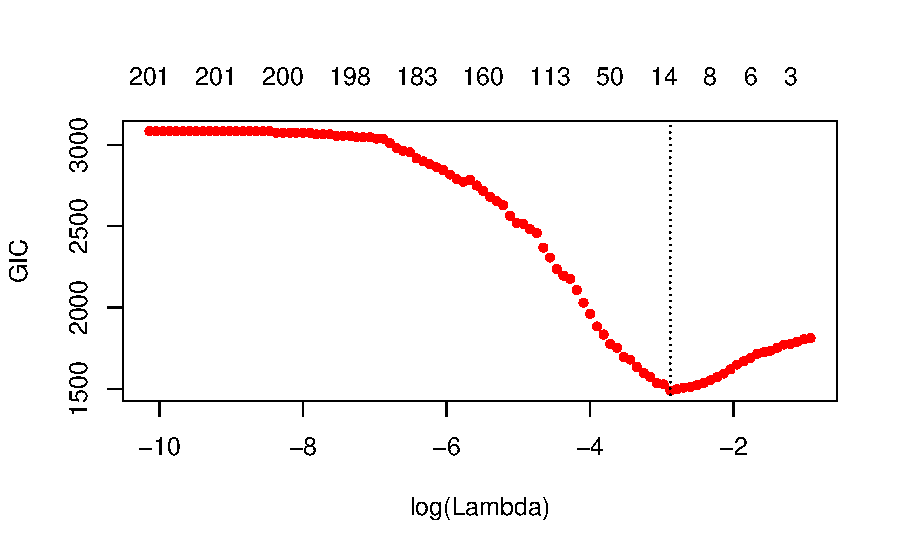
\includegraphics[width=1\linewidth]{figs/ggmix-hdbic-1} 

}



\end{knitrout}

The optimal value for $\lambda$ according to the HDBIC, i.e., the $\lambda$ that leads to the minium HDBIC is:

\begin{knitrout}\scriptsize
\definecolor{shadecolor}{rgb}{0.969, 0.969, 0.969}\color{fgcolor}\begin{kframe}
\begin{alltt}
\hlstd{hdbic[[}\hlstr{"lambda.min"}\hlstd{]]}
\end{alltt}
\begin{verbatim}
## [1] 0.05596623
\end{verbatim}
\end{kframe}
\end{knitrout}


We can also plot the BIC results:

\begin{knitrout}\scriptsize
\definecolor{shadecolor}{rgb}{0.969, 0.969, 0.969}\color{fgcolor}\begin{kframe}
\begin{alltt}
\hlkwd{plot}\hlstd{(bicfit,} \hlkwc{ylab} \hlstd{=} \hlstr{"BIC"}\hlstd{)}
\end{alltt}
\end{kframe}

{\centering 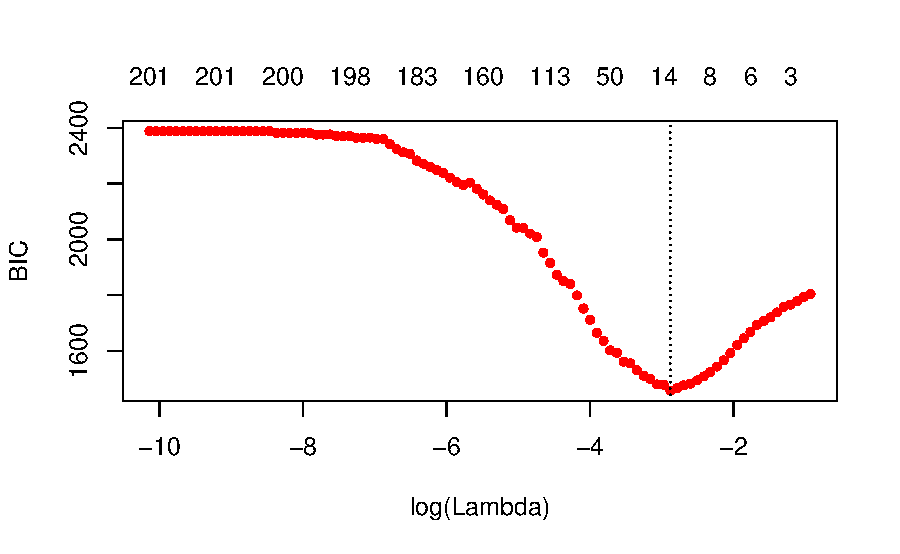
\includegraphics[width=1\linewidth]{figs/ggmix-bic-1} 

}


\begin{kframe}\begin{alltt}
\hlstd{bicfit[[}\hlstr{"lambda.min"}\hlstd{]]}
\end{alltt}
\begin{verbatim}
## [1] 0.05596623
\end{verbatim}
\end{kframe}
\end{knitrout}


\subsection{Get Coefficients Corresponding to Optimal Model}

We can use the object outputted by the \texttt{gic} function to extract the coefficients corresponding to the selected model using the \texttt{coef} method for objects of class \texttt{ggmix\_gic}:  

\begin{knitrout}\scriptsize
\definecolor{shadecolor}{rgb}{0.969, 0.969, 0.969}\color{fgcolor}\begin{kframe}
\begin{alltt}
\hlkwd{coef}\hlstd{(hdbic)[}\hlnum{1}\hlopt{:}\hlnum{5}\hlstd{, ,} \hlkwc{drop} \hlstd{=} \hlnum{FALSE}\hlstd{]}
\end{alltt}
\begin{verbatim}
## 5 x 1 sparse Matrix of class "dgCMatrix"
##                      1
## (Intercept) -0.2668419
## X62          .        
## X185         .        
## X371         .        
## X420         .
\end{verbatim}
\end{kframe}
\end{knitrout}

We can also extract just the nonzero coefficients which also provide the estimated variance components $\eta$ and $\sigma^2$:

\begin{knitrout}\scriptsize
\definecolor{shadecolor}{rgb}{0.969, 0.969, 0.969}\color{fgcolor}\begin{kframe}
\begin{alltt}
\hlkwd{coef}\hlstd{(hdbic,} \hlkwc{type} \hlstd{=} \hlstr{"nonzero"}\hlstd{)}
\end{alltt}
\begin{verbatim}
##                       1
## (Intercept) -0.26684191
## X336        -0.67986393
## X7638        0.43403365
## X1536        0.93994982
## X1943        0.56600730
## X2849       -0.58157979
## X56         -0.08244685
## X4106       -0.35939830
## eta          0.26746240
## sigma2       0.98694300
\end{verbatim}
\end{kframe}
\end{knitrout}

We can also make predictions from the \texttt{hdbic} object, which by default will use the model corresponding to the optimal tuning parameter:

\begin{knitrout}\scriptsize
\definecolor{shadecolor}{rgb}{0.969, 0.969, 0.969}\color{fgcolor}\begin{kframe}
\begin{alltt}
\hlkwd{predict}\hlstd{(hdbic,} \hlkwc{newx} \hlstd{= admixed}\hlopt{$}\hlstd{x[}\hlnum{1}\hlopt{:}\hlnum{5}\hlstd{,])}
\end{alltt}
\begin{verbatim}
##              1
## id1 -1.3061041
## id2  0.2991654
## id3 -2.3453664
## id4 -0.4486012
## id5 -1.3895793
\end{verbatim}
\end{kframe}
\end{knitrout}


\subsection{Extracting Random Effects}

The user can compute the random effects using the provided \texttt{ranef} method for objects of class \texttt{ggmix\_gic}. This command will compute the estimated random effects for each subject using the parameters of the selected model:

\begin{knitrout}\scriptsize
\definecolor{shadecolor}{rgb}{0.969, 0.969, 0.969}\color{fgcolor}\begin{kframe}
\begin{alltt}
\hlkwd{ranef}\hlstd{(hdbic)[}\hlnum{1}\hlopt{:}\hlnum{5}\hlstd{]}
\end{alltt}
\begin{verbatim}
## [1] -0.02548691 -0.10011680  0.13020240 -0.30650997  0.16045768
\end{verbatim}
\end{kframe}
\end{knitrout}



\subsection{Diagnostic Plots}

We can also plot some standard diagnotic plots such as the observed vs. predicted response, QQ-plots of the residuals and random effects and the Tukey-Anscombe plot. These can be plotted using the \texttt{plot} method on a \texttt{ggmix\_gic} object as shown below.


\subsubsection{Observed vs. Predicted Response}

\begin{knitrout}\scriptsize
\definecolor{shadecolor}{rgb}{0.969, 0.969, 0.969}\color{fgcolor}\begin{kframe}
\begin{alltt}
\hlkwd{plot}\hlstd{(hdbic,} \hlkwc{type} \hlstd{=} \hlstr{"predicted"}\hlstd{,} \hlkwc{newx} \hlstd{= admixed}\hlopt{$}\hlstd{x,} \hlkwc{newy} \hlstd{= admixed}\hlopt{$}\hlstd{y)}
\end{alltt}
\end{kframe}

{\centering 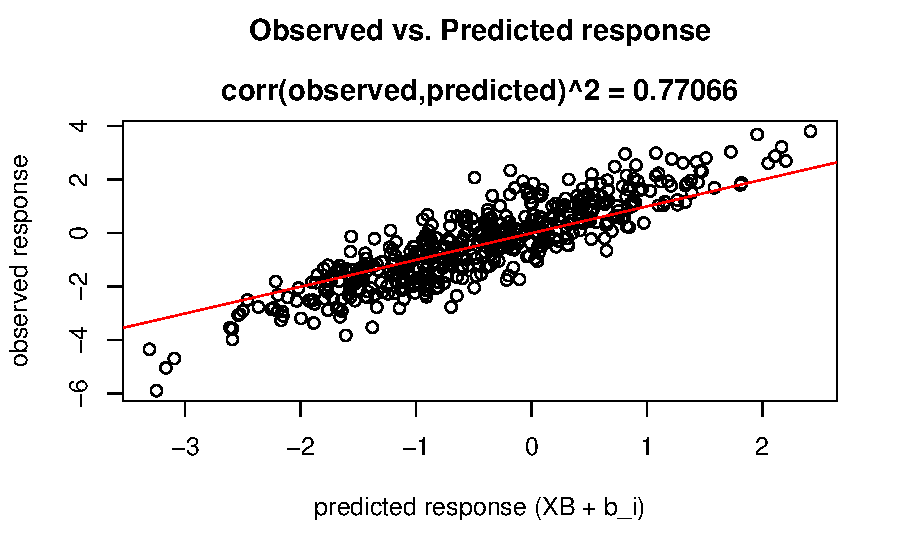
\includegraphics[width=1\linewidth]{figs/ggmix-obs-pred-1} 

}



\end{knitrout}


\subsubsection{QQ-plots for Residuals and Random Effects}

\begin{knitrout}\scriptsize
\definecolor{shadecolor}{rgb}{0.969, 0.969, 0.969}\color{fgcolor}\begin{kframe}
\begin{alltt}
\hlkwd{plot}\hlstd{(hdbic,} \hlkwc{type} \hlstd{=} \hlstr{"QQranef"}\hlstd{,} \hlkwc{newx} \hlstd{= admixed}\hlopt{$}\hlstd{x,} \hlkwc{newy} \hlstd{= admixed}\hlopt{$}\hlstd{y)}
\end{alltt}
\end{kframe}

{\centering 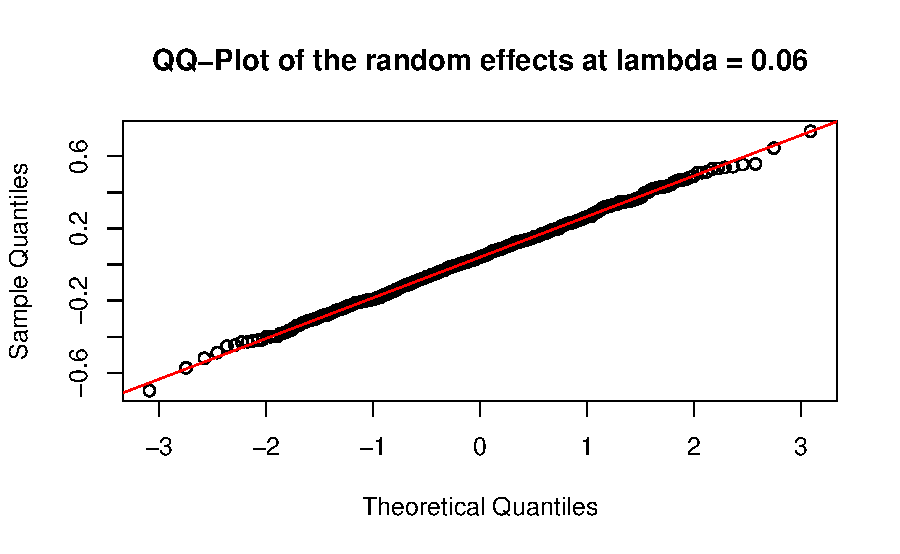
\includegraphics[width=1\linewidth]{figs/ggmix-qqplot-1} 

}


\begin{kframe}\begin{alltt}
\hlkwd{plot}\hlstd{(hdbic,} \hlkwc{type} \hlstd{=} \hlstr{"QQresid"}\hlstd{,} \hlkwc{newx} \hlstd{= admixed}\hlopt{$}\hlstd{x,} \hlkwc{newy} \hlstd{= admixed}\hlopt{$}\hlstd{y)}
\end{alltt}
\end{kframe}

{\centering 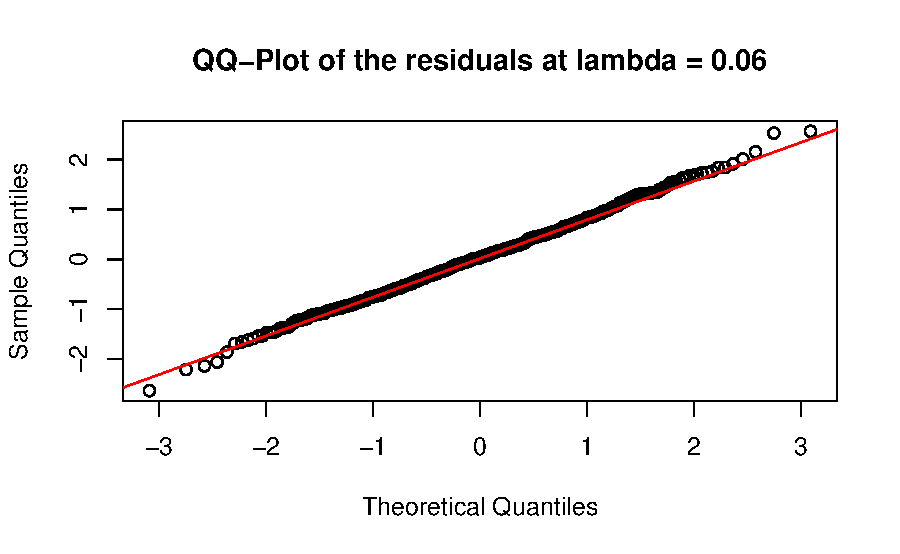
\includegraphics[width=1\linewidth]{figs/ggmix-qqplot-2} 

}



\end{knitrout}


\subsubsection{Tukey-Anscombe Plot}

\begin{knitrout}\scriptsize
\definecolor{shadecolor}{rgb}{0.969, 0.969, 0.969}\color{fgcolor}\begin{kframe}
\begin{alltt}
\hlkwd{plot}\hlstd{(hdbic,} \hlkwc{type} \hlstd{=} \hlstr{"Tukey"}\hlstd{,} \hlkwc{newx} \hlstd{= admixed}\hlopt{$}\hlstd{x,} \hlkwc{newy} \hlstd{= admixed}\hlopt{$}\hlstd{y)}
\end{alltt}
\end{kframe}

{\centering 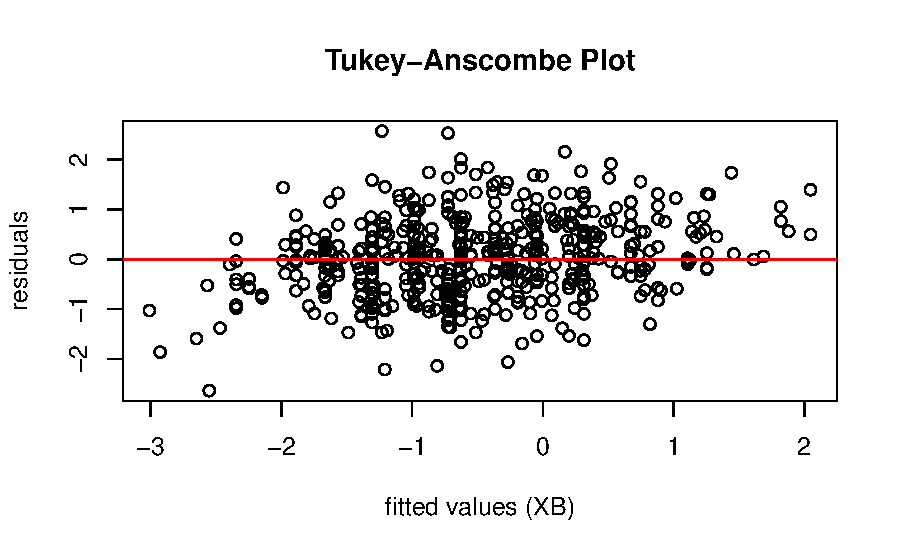
\includegraphics[width=1\linewidth]{figs/ggmix-tukey-1} 

}



\end{knitrout}



